% =====================================================================
% Rapport d'avancement - SkillSeek AI
% Auteur : Aymen Benrbib - ESI (ISITD) - Stage BC SKILLS 2026
% Compilation : pdflatex (Overleaf : compiler "pdfLaTeX", 2 passes)
% IMPORTANT : placer le logo a cote du .tex sous le nom "bc_skills.jpg"
% =====================================================================
\documentclass[11pt,a4paper]{article}

\usepackage[utf8]{inputenc}
\usepackage[T1]{fontenc}
% Francisation : utilise babel-french s'il est installe (Overleaf, TeX Live
% complet), sinon bascule sur une francisation manuelle equivalente afin que
% le document compile dans tous les environnements.
\IfFileExists{french.ldf}{%
  \usepackage[french]{babel}%
}{%
  \renewcommand{\contentsname}{Table des matières}%
  \renewcommand{\figurename}{Figure}%
  \renewcommand{\tablename}{Tableau}%
  \renewcommand{\refname}{Références}%
}
\usepackage{lmodern}
\usepackage[margin=2.4cm]{geometry}
\usepackage{graphicx}
\usepackage{xcolor}
\usepackage{booktabs}
\usepackage{array}
\usepackage{longtable}
\usepackage{enumitem}
\usepackage{titlesec}
\usepackage{fancyhdr}
\usepackage{tikz}
\usepackage{float}      % option [H] : fige les figures a leur place exacte
\usepackage{listings}
\usetikzlibrary{arrows.meta, positioning, shapes.geometric, fit, calc, backgrounds}
\usepackage{hyperref}

\raggedbottom

% ------------------ Couleurs ------------------
\definecolor{primaire}{HTML}{1F3A5F}
\definecolor{accent}{HTML}{2E86AB}
\definecolor{fondclair}{HTML}{EEF4F8}
\definecolor{vert}{HTML}{2E7D5B}
\definecolor{gris}{HTML}{6B7A8F}

\hypersetup{colorlinks=true, linkcolor=primaire, urlcolor=accent,
  pdftitle={Rapport d'avancement - SkillSeek AI}, pdfauthor={Aymen Benrbib}}

% ------------------ Titres ------------------
\titleformat{\section}{\Large\bfseries\color{primaire}}{\thesection}{0.6em}{}
\titlespacing*{\section}{0pt}{14pt}{8pt}
\titleformat{\subsection}{\large\bfseries\color{primaire}}{\thesubsection}{0.6em}{}
\titleformat{\subsubsection}{\normalsize\bfseries\color{accent}}{\thesubsubsection}{0.6em}{}

% ------------------ En-tete / pied ------------------
\pagestyle{fancy}
\fancyhf{}
\fancyhead[L]{\small\color{primaire} Rapport d'avancement -- SkillSeek AI}
\fancyhead[R]{\small\color{primaire} BC SKILLS -- Juillet 2026}
\fancyfoot[C]{\small\thepage}
\renewcommand{\headrulewidth}{0.4pt}

% ------------------ Styles TikZ ------------------
\tikzset{
  bloc/.style={rectangle, rounded corners=2pt, draw=primaire, fill=fondclair,
    text=primaire, font=\small\bfseries, minimum height=8mm,
    minimum width=22mm, align=center, inner sep=1.6mm},
  blocia/.style={bloc, draw=accent, fill=white, text=accent},
  classe/.style={rectangle, draw=primaire, fill=white, font=\scriptsize,
    align=left, inner sep=1.4mm, minimum width=30mm},
  acteur/.style={font=\small, align=center},
  uc/.style={ellipse, draw=accent, fill=fondclair, font=\scriptsize,
    align=center, inner sep=1mm, minimum width=28mm, minimum height=7mm},
  fleche/.style={-{Stealth[length=2.2mm]}, thick, color=primaire},
  lien/.style={thick, color=gris},
  etiquette/.style={font=\scriptsize, color=primaire, align=center},
  vie/.style={dashed, color=gris},
  etape/.style={rectangle, rounded corners=3pt, draw=primaire, fill=fondclair,
    font=\scriptsize, align=center, minimum width=26mm, minimum height=7mm},
  decision/.style={diamond, draw=primaire, fill=white, font=\scriptsize,
    align=center, aspect=2, inner sep=0.8mm}
}

% ------------------ Code source ------------------
\lstset{
  basicstyle=\ttfamily\scriptsize,
  backgroundcolor=\color{fondclair},
  frame=single,
  rulecolor=\color{gris},
  breaklines=true,
  keywordstyle=\color{primaire}\bfseries,
  commentstyle=\color{vert},
  showstringspaces=false,
  language=Python
}

\begin{document}

% =====================================================================
% PAGE DE GARDE
% =====================================================================
\begin{titlepage}
  \centering
  % Logo : placer bc_skills.jpg dans ce dossier. Sans le fichier, un cadre
  % de reservation s'affiche et la compilation reussit quand meme.
  \IfFileExists{bc_skills.jpg}{%
    
\includegraphics[width=4.5cm]{bc_skills.jpg}%
  }{%
    \fbox{\parbox[c][3cm][c]{4.5cm}{\centering\small\color{gris}
      Logo BC SKILLS\\ (ajouter \texttt{bc\_skills.jpg})}}%
  }\\[1cm]
  {\color{primaire}\rule{\textwidth}{2pt}}\\[1cm]
  {\large École des Sciences de l'Information (ESI)}\\[0.2cm]
  {\normalsize Filière : Ingénierie des Systèmes d'Information et Transformation Digitale (ISITD)}\\[2cm]

  {\Huge\bfseries\color{primaire} Rapport d'avancement}\\[0.6cm]
  {\LARGE\bfseries SkillSeek AI}\\[0.8cm]
  {\large Plateforme intelligente de gestion du recrutement\\ Bilan du Sprint 1 et conception détaillée}\\[2.5cm]

  \begin{tabular}{ll}
    \textbf{Auteur :}              & Aymen Benrbib \\[2mm]
    \textbf{Organisme d'accueil :} & BC SKILLS \\
  \end{tabular}\\[2.5cm]

  {\color{primaire}\rule{\textwidth}{2pt}}
\end{titlepage}

\tableofcontents
\newpage

% =====================================================================
\section{Objet du rapport}
% =====================================================================
Ce document présente l'état d'avancement du projet \textbf{SkillSeek AI} à la date du 21 juillet 2026. Il couvre la clôture du Sprint~1, détaille la conception du système à travers les diagrammes UML de référence, présente les réalisations techniques vérifiées, et expose la planification révisée jusqu'à la livraison finale prévue le 16 août 2026.

\subsection{Rappel du projet}
SkillSeek AI est une plateforme web de gestion du recrutement permettant de publier des offres d'emploi, de collecter les candidatures, d'analyser automatiquement les CV, de classer les candidats selon un score de compatibilité et de piloter l'activité via un tableau de bord décisionnel.

% =====================================================================
\section{Synthèse de l'avancement}
% =====================================================================

\subsection{État global}

\begin{center}
\begin{tabular}{lccp{5.2cm}}
  \toprule
  \textbf{Sprint} & \textbf{Période} & \textbf{État} & \textbf{Périmètre} \\
  \midrule
  Sprint 1 & 06/07 -- 15/07 & \textcolor{vert}{\textbf{Terminé}} & Socle technique, base de données, API, sécurité \\[1mm]
  Sprint 2 & 16/07 -- 27/07 & \textcolor{accent}{\textbf{En cours}} & Interface utilisateur, CRUD métier \\[1mm]
  Sprint 3 & 28/07 -- 06/08 & Planifié & Moteur d'analyse des CV et classement \\[1mm]
  Sprint 4 & 07/08 -- 16/08 & Planifié & Assistant conversationnel, tableau de bord, Power BI \\
  \bottomrule
\end{tabular}
\end{center}

\vspace{2mm}
\noindent Avancement global estimé : \textbf{25\,\%} du périmètre fonctionnel, correspondant à 100\,\% du socle technique.

\subsection{Tâches du Sprint 1}

\begin{center}
\begin{tabular}{clp{6.6cm}c}
  \toprule
  \textbf{ID} & \textbf{Tâche} & \textbf{Livrable vérifié} & \textbf{État} \\
  \midrule
  S1-01 & Dépôt Git & Monorepo structuré, branches \texttt{main}/\texttt{dev} & \textcolor{vert}{OK} \\
  S1-02 & Conteneurisation & \texttt{docker-compose} : PostgreSQL + API & \textcolor{vert}{OK} \\
  S1-03 & Pipeline CI/CD & GitHub Actions : lint + tests automatiques & \textcolor{vert}{OK} \\
  S1-04 & Modélisation BDD & 7 entités, migrations Alembic & \textcolor{vert}{OK} \\
  S1-05 & Architecture API & Factory Flask, 4 Blueprints & \textcolor{vert}{OK} \\
  S1-06 & Authentification & JWT, refresh, révocation, bcrypt & \textcolor{vert}{OK} \\
  S1-07 & RBAC temps réel & Middleware de vérification des droits & \textcolor{vert}{OK} \\
  \bottomrule
\end{tabular}
\end{center}

% =====================================================================
\section{Conception du système (UML)}
% =====================================================================

\subsection{Diagramme de cas d'utilisation}
La figure~\ref{fig:uc} présente les fonctionnalités offertes à chaque catégorie d'utilisateur.

\begin{figure}[H]
  \centering
  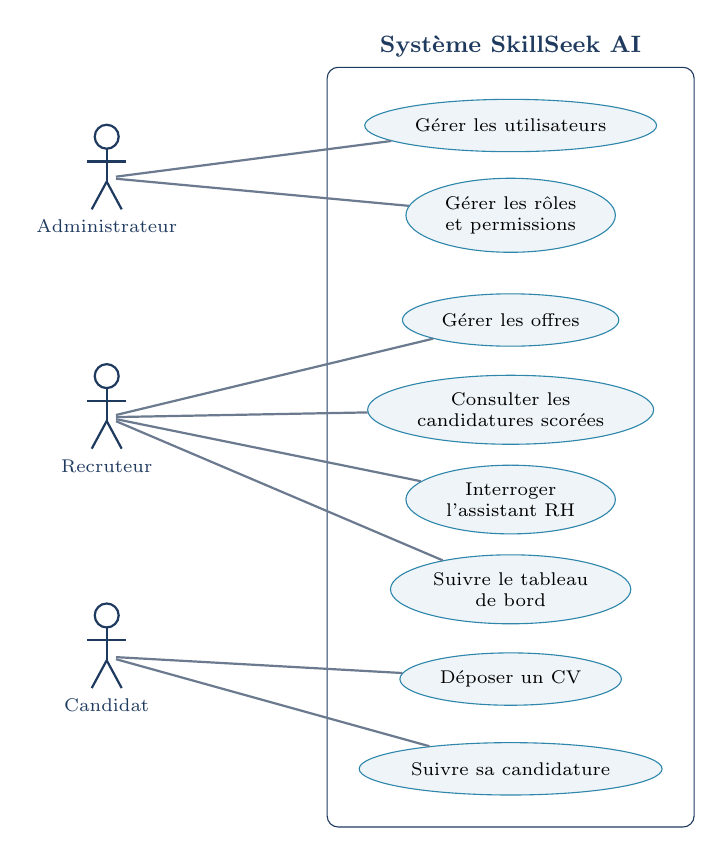
\begin{tikzpicture}[scale=0.95, transform shape]
    % Acteurs (bonhommes dessines en TikZ)
    \foreach \y/\nom/\id in {0/Administrateur/adm, -3.2/Recruteur/rec, -6.4/Candidat/can} {
      \begin{scope}[shift={(0, \y)}, color=primaire, thick]
        \draw (0, 0.55) circle (0.16);
        \draw (0, 0.39) -- (0, -0.05);
        \draw (-0.26, 0.22) -- (0.26, 0.22);
        \draw (0, -0.05) -- (-0.2, -0.42);
        \draw (0, -0.05) -- (0.2, -0.42);
        \node[font=\scriptsize, color=primaire] at (0, -0.65) {\nom};
      \end{scope}
      \node (\id) at (0, \y) {};
    }

    % Cas d'utilisation
    \node[uc] (uc1) at (5.4, 0.7)  {Gérer les utilisateurs};
    \node[uc] (uc2) at (5.4, -0.5) {Gérer les rôles\\ et permissions};
    \node[uc] (uc3) at (5.4, -1.9) {Gérer les offres};
    \node[uc] (uc4) at (5.4, -3.1) {Consulter les\\ candidatures scorées};
    \node[uc] (uc5) at (5.4, -4.3) {Interroger\\ l'assistant RH};
    \node[uc] (uc6) at (5.4, -5.5) {Suivre le tableau\\ de bord};
    \node[uc] (uc7) at (5.4, -6.7) {Déposer un CV};
    \node[uc] (uc8) at (5.4, -7.9) {Suivre sa candidature};

    \draw[lien] (adm) -- (uc1);
    \draw[lien] (adm) -- (uc2);
    \draw[lien] (rec) -- (uc3);
    \draw[lien] (rec) -- (uc4);
    \draw[lien] (rec) -- (uc5);
    \draw[lien] (rec) -- (uc6);
    \draw[lien] (can) -- (uc7);
    \draw[lien] (can) -- (uc8);

    % Frontiere du systeme
    \begin{scope}[on background layer]
      \node[draw=primaire, rounded corners, fit=(uc1)(uc8), inner sep=4mm,
            label={[font=\small\bfseries, color=primaire]above:Système SkillSeek AI}] {};
    \end{scope}
  \end{tikzpicture}
  \caption{Diagramme de cas d'utilisation.}
  \label{fig:uc}
\end{figure}

\subsection{Diagramme de classes}
La figure~\ref{fig:classes} présente le modèle de données implémenté au Sprint~1.

\begin{figure}[H]
  \centering
  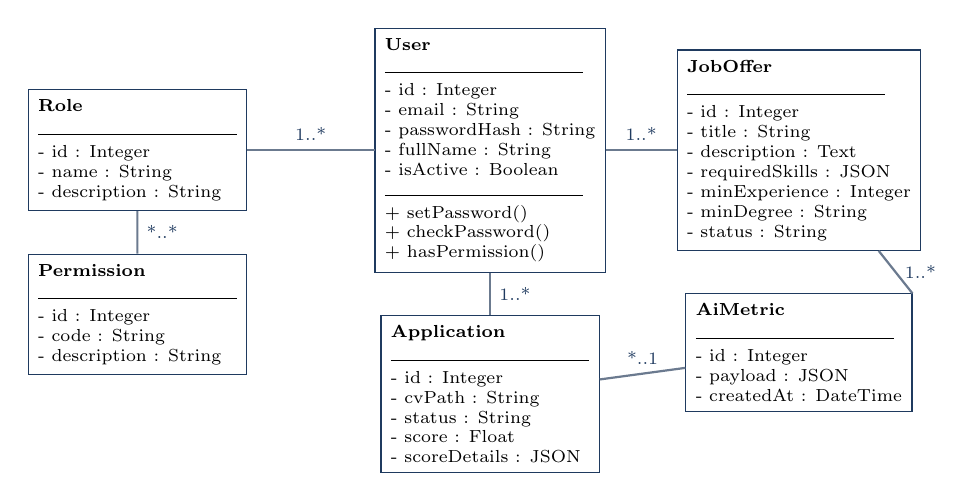
\begin{tikzpicture}[node distance=6mm and 10mm, scale=0.9, transform shape]

    \node[classe] (user) {
      \textbf{User}\\[0.4mm] \rule{28mm}{0.3pt} \\[0.4mm]
      - id : Integer\\
      - email : String\\
      - passwordHash : String\\
      - fullName : String\\
      - isActive : Boolean\\
      \rule{28mm}{0.3pt} \\[0.4mm]
      + setPassword()\\
      + checkPassword()\\
      + hasPermission()
    };

    \node[classe, left=18mm of user] (role) {
      \textbf{Role}\\[0.4mm] \rule{28mm}{0.3pt} \\[0.4mm]
      - id : Integer\\
      - name : String\\
      - description : String
    };

    \node[classe, below=of role] (perm) {
      \textbf{Permission}\\[0.4mm] \rule{28mm}{0.3pt} \\[0.4mm]
      - id : Integer\\
      - code : String\\
      - description : String
    };

    \node[classe, right=of user] (offer) {
      \textbf{JobOffer}\\[0.4mm] \rule{28mm}{0.3pt} \\[0.4mm]
      - id : Integer\\
      - title : String\\
      - description : Text\\
      - requiredSkills : JSON\\
      - minExperience : Integer\\
      - minDegree : String\\
      - status : String
    };

    \node[classe, below=of user] (app) {
      \textbf{Application}\\[0.4mm] \rule{28mm}{0.3pt} \\[0.4mm]
      - id : Integer\\
      - cvPath : String\\
      - status : String\\
      - score : Float\\
      - scoreDetails : JSON
    };

    \node[classe, below=of offer] (metric) {
      \textbf{AiMetric}\\[0.4mm] \rule{28mm}{0.3pt} \\[0.4mm]
      - id : Integer\\
      - payload : JSON\\
      - createdAt : DateTime
    };

    \draw[lien] (role) -- node[etiquette, above]{1..*} (user);
    \draw[lien] (role) -- node[etiquette, right]{*..*} (perm);
    \draw[lien] (user) -- node[etiquette, right]{1..*} (app);
    \draw[lien] (offer) -- node[etiquette, right]{1..*} (metric.north east);
    \draw[lien] (app) -- node[etiquette, above]{*..1} (metric);
    \draw[lien] (user.east) -- node[etiquette, above]{1..*} (offer.west);
  \end{tikzpicture}
  \caption{Diagramme de classes du modèle de données.}
  \label{fig:classes}
\end{figure}

\subsection{Diagramme de séquence : authentification et contrôle des droits}
La figure~\ref{fig:seq} illustre le mécanisme central du Sprint~1 : la vérification des permissions en base à chaque requête sensible, garantissant l'effet immédiat d'une révocation (règle RG-02).

\begin{figure}[H]
  \centering
  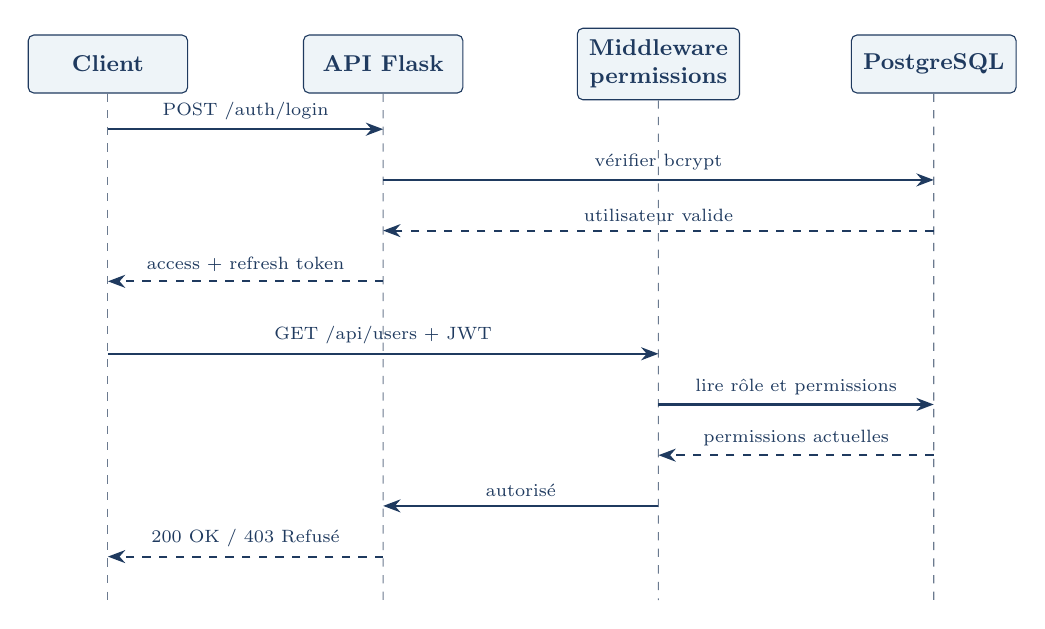
\begin{tikzpicture}[scale=0.92, transform shape]
    % Participants
    \node[bloc] (c) at (0, 0)     {Client};
    \node[bloc] (a) at (3.8, 0)   {API Flask};
    \node[bloc] (m) at (7.6, 0)   {Middleware\\ permissions};
    \node[bloc] (d) at (11.4, 0)  {PostgreSQL};

    % Lignes de vie
    \foreach \n in {c, a, m, d} { \draw[vie] (\n) -- ++(0, -7.4); }

    % Messages
    \draw[fleche] (0, -0.9) -- node[etiquette, above]{\scriptsize POST /auth/login} (3.8, -0.9);
    \draw[fleche] (3.8, -1.6) -- node[etiquette, above]{\scriptsize vérifier bcrypt} (11.4, -1.6);
    \draw[fleche, dashed] (11.4, -2.3) -- node[etiquette, above]{\scriptsize utilisateur valide} (3.8, -2.3);
    \draw[fleche, dashed] (3.8, -3.0) -- node[etiquette, above]{\scriptsize access + refresh token} (0, -3.0);

    \draw[fleche] (0, -4.0) -- node[etiquette, above]{\scriptsize GET /api/users + JWT} (7.6, -4.0);
    \draw[fleche] (7.6, -4.7) -- node[etiquette, above]{\scriptsize lire rôle et permissions} (11.4, -4.7);
    \draw[fleche, dashed] (11.4, -5.4) -- node[etiquette, above]{\scriptsize permissions actuelles} (7.6, -5.4);
    \draw[fleche] (7.6, -6.1) -- node[etiquette, above]{\scriptsize autorisé} (3.8, -6.1);
    \draw[fleche, dashed] (3.8, -6.8) -- node[etiquette, above]{\scriptsize 200 OK / 403 Refusé} (0, -6.8);
  \end{tikzpicture}
  \caption{Diagramme de séquence : connexion puis accès à une ressource protégée.}
  \label{fig:seq}
\end{figure}

\subsection{Diagramme d'activité : traitement d'une candidature}
La figure~\ref{fig:activite} décrit le workflow complet prévu, du dépôt du CV à la décision du recruteur.

\begin{figure}[H]
  \centering
  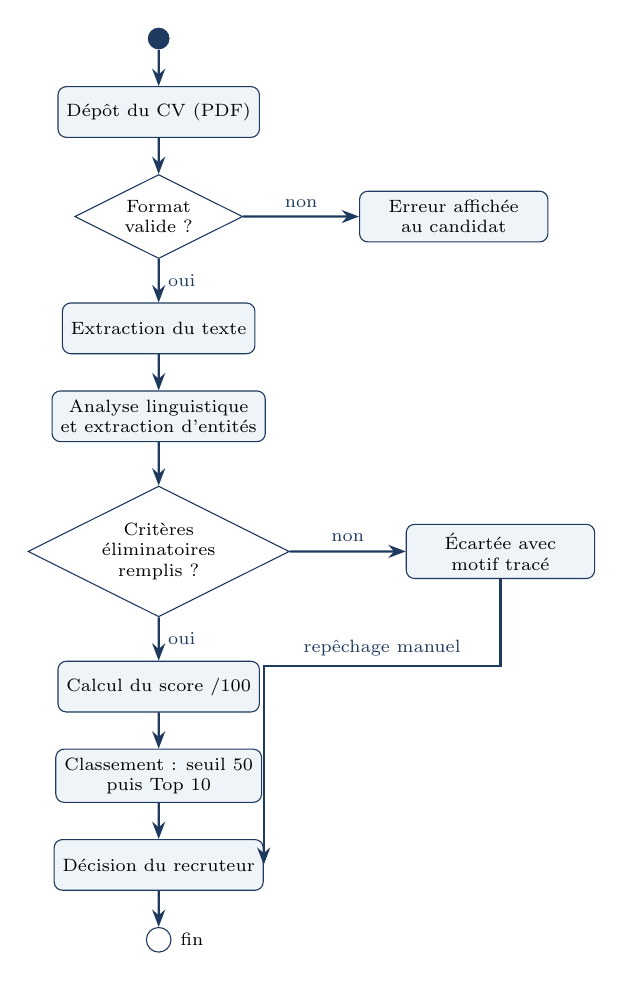
\begin{tikzpicture}[node distance=5mm and 9mm, scale=0.92, transform shape]
    \node[circle, fill=primaire, minimum size=3mm, inner sep=0] (start) {};
    \node[etape, below=of start] (depot) {Dépôt du CV (PDF)};
    \node[decision, below=of depot] (fmt) {Format\\ valide ?};
    \node[etape, below=6mm of fmt] (extract) {Extraction du texte};
    \node[etape, below=of extract] (nlp) {Analyse linguistique\\ et extraction d'entités};
    \node[decision, below=6mm of nlp] (regles) {Critères\\ éliminatoires\\ remplis ?};
    \node[etape, below=6mm of regles] (score) {Calcul du score /100};
    \node[etape, below=of score] (classe) {Classement : seuil 50\\ puis Top 10};
    \node[etape, below=of classe] (dec) {Décision du recruteur};
    \node[circle, draw=primaire, fill=white, minimum size=3.4mm, inner sep=0,
          label=right:{\scriptsize fin}, below=of dec] (end) {};

    \node[etape, right=16mm of fmt] (rejet1) {Erreur affichée\\ au candidat};
    \node[etape, right=16mm of regles] (rejet2) {Écartée avec\\ motif tracé};

    \draw[fleche] (start) -- (depot);
    \draw[fleche] (depot) -- (fmt);
    \draw[fleche] (fmt) -- node[etiquette, right]{oui} (extract);
    \draw[fleche] (fmt) -- node[etiquette, above]{non} (rejet1);
    \draw[fleche] (extract) -- (nlp);
    \draw[fleche] (nlp) -- (regles);
    \draw[fleche] (regles) -- node[etiquette, right]{oui} (score);
    \draw[fleche] (regles) -- node[etiquette, above]{non} (rejet2);
    \draw[fleche] (score) -- (classe);
    \draw[fleche] (classe) -- (dec);
    \draw[fleche] (dec) -- (end);
    \draw[fleche] (rejet2.south) |- ++(0, -1.2) -| node[etiquette, above, pos=0.25]{repêchage manuel} (dec.east);
  \end{tikzpicture}
  \caption{Diagramme d'activité : cycle de vie d'une candidature.}
  \label{fig:activite}
\end{figure}

\subsection{Diagramme de composants}
La figure~\ref{fig:composants} présente l'organisation modulaire de l'application.

\begin{figure}[H]
  \centering
  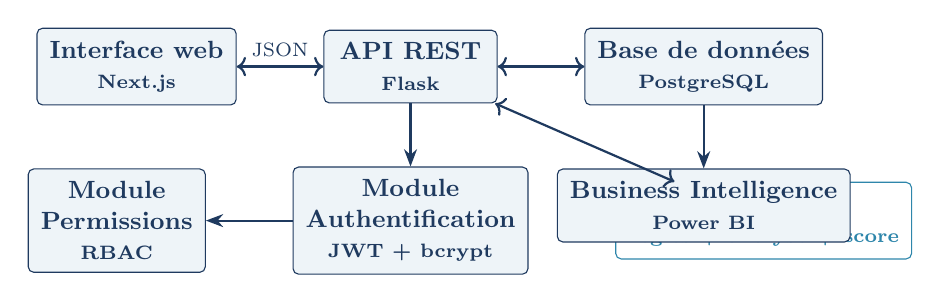
\begin{tikzpicture}[node distance=8mm and 11mm]
    \node[bloc] (front) {Interface web\\ \scriptsize Next.js};
    \node[bloc, right=of front] (api) {API REST\\ \scriptsize Flask};
    \node[bloc, right=of api] (db) {Base de données\\ \scriptsize PostgreSQL};
    \node[bloc, below=of api] (auth) {Module\\ Authentification\\ \scriptsize JWT + bcrypt};
    \node[bloc, left=of auth] (rbac) {Module\\ Permissions\\ \scriptsize RBAC};
    \node[blocia, right=of auth] (ia) {Module IA\\ \scriptsize règles + analyse + score};
    \node[bloc, below=of db] (bi) {Business Intelligence\\ \scriptsize Power BI};

    \draw[fleche, <->] (front) -- node[etiquette, above]{\scriptsize JSON} (api);
    \draw[fleche, <->] (api) -- (db);
    \draw[fleche] (api) -- (auth);
    \draw[fleche] (auth) -- (rbac);
    \draw[fleche, <->] (api) -- (ia);
    \draw[fleche] (db) -- (bi);
  \end{tikzpicture}
  \caption{Diagramme de composants de la plateforme.}
  \label{fig:composants}
\end{figure}

\subsection{Diagramme de déploiement}
La figure~\ref{fig:deploiement} montre la répartition des composants dans l'environnement conteneurisé.

\begin{figure}[H]
  \centering
  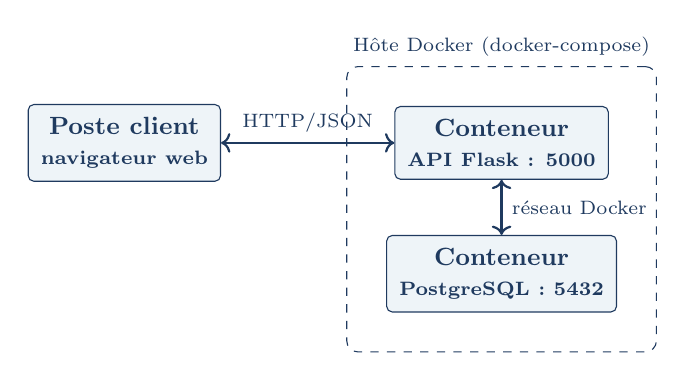
\begin{tikzpicture}[node distance=7mm and 12mm]
    \node[bloc] (nav) {Poste client\\ \scriptsize navigateur web};
    \node[bloc, right=22mm of nav] (capi) {Conteneur\\ \scriptsize API Flask : 5000};
    \node[bloc, below=of capi] (cdb) {Conteneur\\ \scriptsize PostgreSQL : 5432};

    \draw[fleche, <->] (nav) -- node[etiquette, above]{\scriptsize HTTP/JSON} (capi);
    \draw[fleche, <->] (capi) -- node[etiquette, right]{\scriptsize réseau Docker} (cdb);

    \begin{scope}[on background layer]
      \node[draw=primaire, dashed, rounded corners, fit=(capi)(cdb), inner sep=5mm,
            label={[font=\scriptsize, color=primaire]above:Hôte Docker (docker-compose)}] {};
    \end{scope}
  \end{tikzpicture}
  \caption{Diagramme de déploiement de l'environnement actuel.}
  \label{fig:deploiement}
\end{figure}

% =====================================================================
\section{Réalisations du Sprint 1}
% =====================================================================

\subsection{Socle technique et industrialisation}
Le projet est organisé en dépôt unique structuré, avec deux branches de travail (\texttt{main} pour les versions stables, \texttt{dev} pour le développement courant). L'ensemble de l'environnement est conteneurisé : une seule commande démarre simultanément la base de données et l'API, garantissant un comportement identique sur tout poste de travail.

Une chaîne d'intégration continue est en place : chaque envoi de code déclenche automatiquement une analyse de qualité (\texttt{flake8}) puis l'exécution de la suite de tests. Un échec bloque l'intégration, ce qui empêche toute régression d'atteindre la branche principale.

\subsection{Modèle de données}
Sept entités ont été modélisées et migrées : \texttt{User}, \texttt{Role}, \texttt{Permission} (avec table d'association pour le RBAC dynamique), \texttt{JobOffer}, \texttt{Application}, \texttt{AiMetric} et \texttt{TokenBlocklist}. Le modèle anticipe les besoins des sprints suivants : les critères éliminatoires sont portés par l'offre, et la candidature dispose des champs \texttt{score} et \texttt{scoreDetails} destinés au classement et à son explication.

\subsection{Architecture applicative}
L'API suit le patron \emph{factory} avec une organisation en modules fonctionnels (\emph{Blueprints}) : authentification, utilisateurs, offres et candidatures. La configuration est externalisée par environnement (développement, test, production), et la gestion des erreurs est centralisée afin de renvoyer des réponses homogènes.

\subsection{Sécurité}
Les mesures suivantes sont opérationnelles :
\begin{itemize}[leftmargin=1.5em, nosep]
  \item mots de passe hachés avec \texttt{bcrypt}, jamais stockés en clair ;
  \item jetons d'accès à durée courte (15 minutes) associés à un jeton de rafraîchissement ;
  \item table de révocation permettant d'invalider immédiatement une session ;
  \item validation stricte des entrées (format d'email, robustesse du mot de passe) ;
  \item accès aux données exclusivement via une couche d'abstraction, prévenant les injections SQL ;
  \item messages d'erreur indifférenciés à la connexion, empêchant l'énumération des comptes.
\end{itemize}

\subsection{Contrôle d'accès en temps réel}
Le mécanisme retenu constitue un point différenciant du projet. Le jeton d'authentification ne transporte que l'identité de l'utilisateur ; ses permissions sont relues en base de données à chaque requête sensible. Lorsqu'un administrateur retire un droit, la restriction s'applique dès la requête suivante, sans attendre l'expiration du jeton.

\begin{lstlisting}[caption={Décorateur de contrôle des permissions.}]
def require_permission(*codes):
    def decorator(fn):
        @wraps(fn)
        def wrapper(*args, **kwargs):
            verify_jwt_in_request()
            user = _load_current_user()          # relecture en base
            if user is None or not user.is_active:
                return jsonify(error="Compte inexistant ou desactive."), 401
            missing = [c for c in codes if not user.has_permission(c)]
            if missing:
                return jsonify(error="Permission refusee."), 403
            return fn(user, *args, **kwargs)
        return wrapper
    return decorator
\end{lstlisting}

\subsection{Vérification par les tests}
Une suite de neuf tests automatisés valide le socle : accessibilité du service, création de compte, refus des mots de passe faibles, rejet des identifiants erronés, consultation du profil, révocation de session, autorisation de l'administrateur, refus d'un utilisateur non habilité, et surtout \textbf{effet immédiat du retrait d'une permission}. Ce dernier test constitue la preuve formelle de la règle de gestion RG-02.

\begin{center}
\begin{tabular}{lcc}
  \toprule
  \textbf{Suite de tests} & \textbf{Nombre} & \textbf{Résultat} \\
  \midrule
  Authentification & 6 & \textcolor{vert}{Réussis} \\
  Contrôle d'accès & 3 & \textcolor{vert}{Réussis} \\
  \midrule
  \textbf{Total} & \textbf{9} & \textcolor{vert}{\textbf{100 \%}} \\
  \bottomrule
\end{tabular}
\end{center}

% =====================================================================
\section{Travaux en cours : Sprint 2}
% =====================================================================
Le Sprint~2 est engagé depuis le 16 juillet. La conception de l'interface est en cours. Un référentiel de conception a été rédigé, précisant pour chacun des quatorze écrans de l'application : sa structure, ses composants, ses états (vide, chargement, erreur) et ses messages. Il fixe également la charte visuelle (thème sombre, palette, typographie) et applique les critères ergonomiques de Bastien et Scapin retenus dans le cahier des charges : guidage explicite de l'utilisateur, concision des écrans pour limiter la charge cognitive, et traitement clair des erreurs.

Les écrans couverts sont : connexion, inscription, liste et détail des offres, dépôt de candidature, suivi de candidature, tableau de bord décisionnel, gestion des offres, consultation des candidatures classées avec panneau d'explication du score, assistant conversationnel, gestion des utilisateurs, gestion des rôles et permissions, profil utilisateur, et pages d'erreur.

% =====================================================================
\section{Planification révisée}
% =====================================================================
Le stage a débuté le 6 juillet 2026 et la livraison finale est fixée au 16 août 2026. Le projet est organisé en quatre sprints de durée homogène (dix à douze jours), permettant une démonstration fonctionnelle à l'issue de chacun.

\begin{center}
\begin{tabular}{clcc}
  \toprule
  \textbf{Sprint} & \textbf{Contenu} & \textbf{Période} & \textbf{Durée} \\
  \midrule
  1 & Socle technique, base de données, API, sécurité & 06/07 -- 15/07 & 10 jours \\
  2 & Interface utilisateur, CRUD offres et candidatures & 16/07 -- 27/07 & 12 jours \\
  3 & Analyse des CV, règles métiers, classement & 28/07 -- 06/08 & 10 jours \\
  4 & Assistant conversationnel, tableau de bord, Power BI & 07/08 -- 16/08 & 10 jours \\
  \bottomrule
\end{tabular}
\end{center}

\vspace{2mm}
\noindent Le respect de ce calendrier est facilité par l'anticipation réalisée durant le Sprint~1 : le modèle de données couvre déjà les besoins des sprints suivants et l'ensemble des écrans a été spécifié dès l'ouverture du Sprint~2.

\begin{figure}[H]
  \centering
  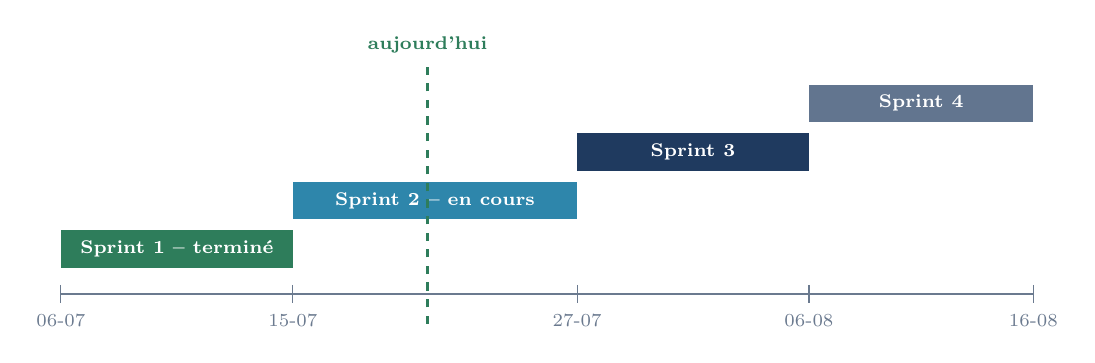
\begin{tikzpicture}[scale=0.95, transform shape]
    % Axe
    \draw[gris, thick] (0,0) -- (13,0);
    \foreach \x/\lab in {0/06-07, 3.1/15-07, 6.9/27-07, 10/06-08, 13/16-08} {
      \draw[gris] (\x, 0.12) -- (\x, -0.12);
      \node[font=\scriptsize, color=gris, below] at (\x, -0.15) {\lab};
    }
    % Barres
    \fill[vert] (0, 0.35) rectangle (3.1, 0.85);
    \node[white, font=\scriptsize\bfseries] at (1.55, 0.6) {Sprint 1 -- terminé};
    \fill[accent] (3.1, 1.0) rectangle (6.9, 1.5);
    \node[white, font=\scriptsize\bfseries] at (5.0, 1.25) {Sprint 2 -- en cours};
    \fill[primaire] (6.9, 1.65) rectangle (10, 2.15);
    \node[white, font=\scriptsize\bfseries] at (8.45, 1.9) {Sprint 3};
    \fill[primaire!70] (10, 2.3) rectangle (13, 2.8);
    \node[white, font=\scriptsize\bfseries] at (11.5, 2.55) {Sprint 4};
    % Jalon aujourd'hui (21/07)
    \draw[dashed, thick, color=vert] (4.9, -0.4) -- (4.9, 3.1);
    \node[font=\scriptsize\bfseries, color=vert, above] at (4.9, 3.1) {aujourd'hui};
  \end{tikzpicture}
  \caption{Planning révisé du projet (diagramme de Gantt simplifié).}
  \label{fig:gantt}
\end{figure}

% =====================================================================
\section{Risques identifiés et mesures}
% =====================================================================

\begin{center}
\begin{tabular}{p{4.6cm}cp{7.4cm}}
  \toprule
  \textbf{Risque} & \textbf{Criticité} & \textbf{Mesure retenue} \\
  \midrule
  Densité du Sprint 4 (assistant, tableau de bord, Power BI) & Élevée & Priorisation stricte : le classement des candidatures et le tableau de bord priment sur le déploiement distant, remplaçable par une démonstration conteneurisée locale. \\[1mm]
  Constitution du jeu de données d'apprentissage & Élevée & Solution de repli : classement fondé sur la similarité sémantique seule, sans apprentissage supervisé, si le corpus s'avère insuffisant. \\[1mm]
  Qualité variable des CV (documents scannés) & Moyenne & Extraction native en premier choix, reconnaissance optique de caractères en solution de repli. \\[1mm]
  Coût des services externes & Faible & Sélection exclusive d'outils gratuits ou en licence libre pour l'ensemble de la chaîne. \\
  \bottomrule
\end{tabular}
\end{center}

% =====================================================================
\section{Conclusion}
% =====================================================================
Le Sprint~1 a été clôturé le 15 juillet 2026, conformément au plan initial. Le socle technique est opérationnel et vérifié par une suite de tests automatisés : environnement conteneurisé reproductible, chaîne d'intégration continue active, modèle de données complet, et couche de sécurité incluant un contrôle d'accès appliqué en temps réel.

Le Sprint~2, engagé depuis le 16 juillet, se déroule dans de bonnes conditions : la conception de l'interface est avancée et l'ensemble des écrans est spécifié. Les prochains travaux porteront sur la réalisation de l'interface utilisateur et la mise en œuvre des parcours métier, avant d'aborder le cœur analytique du projet lors du Sprint~3.

\end{document}
